\documentclass{article}
\usepackage{amsmath,amsfonts,amsthm,amssymb,amsopn,bm}
\usepackage[margin=.9in]{geometry}
\usepackage{graphicx}
\usepackage{url}
\usepackage[usenames,dvipsnames]{color}
\usepackage{fancyhdr}
\usepackage{multirow}
\usepackage{listings}
\usepackage{hyperref}

\definecolor{keywords}{RGB}{255,0,90}
\definecolor{comments}{RGB}{0,0,113}
\definecolor{red}{RGB}{160,0,0}
\definecolor{green}{RGB}{0,150,0}
 
\lstset{language=Python, 
        basicstyle=\ttfamily\tiny, 
        keywordstyle=\color{keywords},
        commentstyle=\color{comments},
        stringstyle=\color{red},
        showstringspaces=false}

\newcommand{\field}[1]{\mathbb{#1}}
\newcommand{\1}{\mathbf{1}}
\newcommand{\E}{\mathbb{E}} 
\newcommand{\Z}{\mathbb{Z}} 
\renewcommand{\P}{\mathbb{P}}
\newcommand{\R}{\field{R}} % real domain
% \newcommand{\C}{\field{C}} % complex domain
\newcommand{\F}{\field{F}} % functional domain
\newcommand{\T}{^{\textrm T}} % transpose
\def\diag{\text{diag}}

%% operator in linear algebra, functional analysis
\newcommand{\inner}[2]{#1\cdot #2}
\newcommand{\norm}[1]{\left\|#1\right\|}
\newcommand{\twonorm}[1]{\|#1\|_2^2}
% operator in functios, maps such as M: domain1 --> domain 2
\newcommand{\Map}[1]{\mathcal{#1}}
\renewcommand{\theenumi}{\alph{enumi}} 

\newcommand{\Perp}{\perp \! \! \! \perp}

\newcommand\independent{\protect\mathpalette{\protect\independenT}{\perp}}
\def\independenT#1#2{\mathrel{\rlap{$#1#2$}\mkern2mu{#1#2}}}
\newcommand{\vct}[1]{\boldsymbol{#1}} % vector
\newcommand{\mat}[1]{\boldsymbol{#1}} % matrix
\newcommand{\cst}[1]{\mathsf{#1}} % constant
\newcommand{\ProbOpr}[1]{\mathbb{#1}}
\newcommand{\points}[1]{\small\textcolor{magenta}{\emph{[#1 points]}} \normalsize}
\date{{}}

\setlength\parindent{0px}

\begin{document}
\title{Homework \#2}
\author{\normalsize{Winter 2020, STATS 509}\\
\normalsize{Dino Bektesevic}}
\maketitle

\section*{Problem 1}
\begin{enumerate}
	\item in this case k=1 so the winnings can only be 0 or 2/3, i.e. $X_1=\{0, 2/3\}$. The probability of each coin toss is 1/2. We can write the pmf function as:
	$$f(x) = \begin{cases} 
	        1/2 &\mbox{if } x \in X_1 \\
            0 & \mbox{if } x \notin X_1 
        \end{cases} 
    $$
    essentially saying that the probability of seeing random variable $x$ be either win or lose is 50 percent. the cumulative distribution function, i.e. cdf, is given by $F_X(x) = P(X\leq x) = \sum_i p(x_i)$. In our case this boils down to three cases, corresponding to the two mass points - a win or no win:
	$$F(x) = \begin{cases} 
	        0 &\mbox{if } x < 0 \\
	        1/2 &\mbox{if } 0 \leq x \leq 2/3 \\
            1 & \mbox{if } x > 2/3 
        \end{cases} 
    $$

    \item in case of k=2 there are 4 different winnings $X_2=\{0, 2/3, 2/9, 8/9\}$ corresponding to four outcome cases (where ordering matters) $x=\{tt, ht, th, hh\} = \{\mbox{0+0}, \mbox{2/3+0}, \mbox{0+2/9}, \mbox{2/3+2/9}\}$. The probability of each outcome is 1/4 because these are two independent events each with probability of 1/2. Written down:
    $$f(x) = \begin{cases} 
	        1/4 &\mbox{if } x \in X_2 \\
            0 & \mbox{if } x \notin X_2 
        \end{cases} 
    $$
	Similarly there are now 5 cases corresponding to the 4 mass points in the cdf:
	$$F(x) = \begin{cases} 
	        0 &\mbox{if } x < 0 \\
	        0.25 &\mbox{if } 0\leq x \leq 2/9 \\
            0.5  & \mbox{if } 2/9 < x \leq 2/3 \\
            0.75 & \mbox{if } 2/3 < x \leq 8/9 \\
            1 & \mbox{if } x > 8/9
        \end{cases} 
    $$
	
	\newpage
	\item I run a million simulations counting up all the winnings from each toss in each simulation in Python.
	\begin{center}
    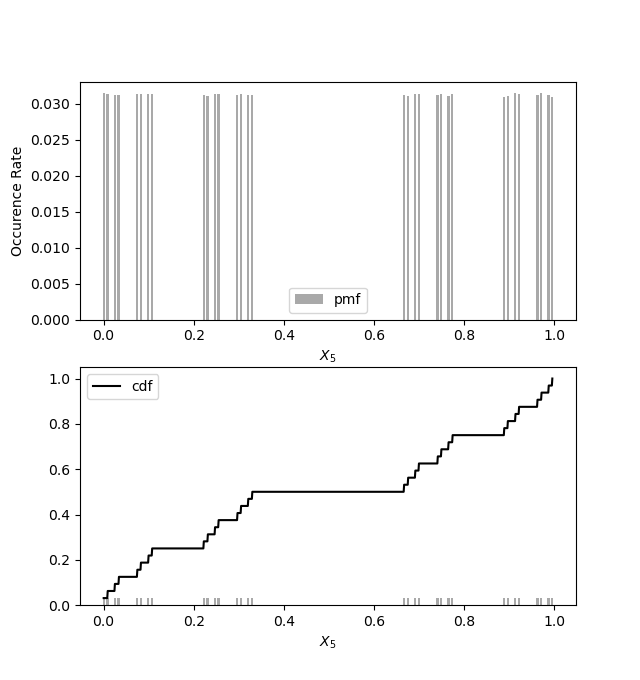
\includegraphics[width=2.5in]{STATS509/HW2/HW2Figures/problem1c.png}
    \end{center}
    \lstinputlisting[language=Python]{HW2Code/HW2_Problem1.py}
\end{enumerate}


\newpage
\section*{Problem 2}
\begin{center}
    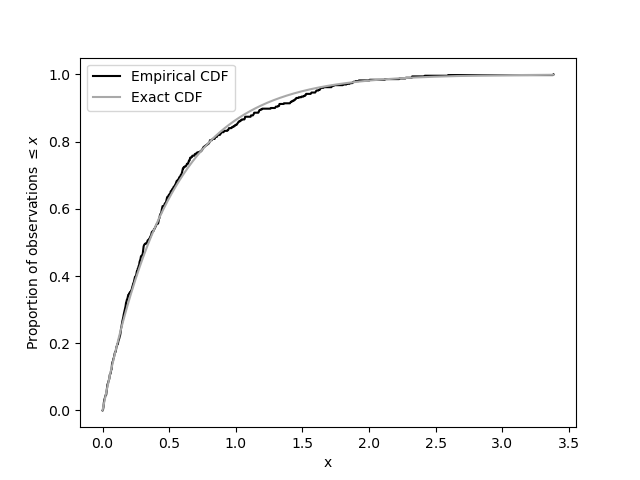
\includegraphics[width=3in]{STATS509/HW2/HW2Figures/problem2.png}
\end{center}
\lstinputlisting[language=Python]{HW2Code/problem2.py}


\newpage
\section*{Problem 3}
\begin{enumerate}
	\item As in all the problems above the empirical CDF is just a counting function:
	$$\F(t) = \frac{1}{n}\sum_{i=1}^n \1\{x_i\leq t\}$$
	
	\item I assume Rectangular distribution is the Uniform distribution given by:
	$$ f(x)=\begin{cases}
            \frac{1}{b - a} & \mathrm{for}\ a \le x \le b, \\
            0 & \mathrm{for}\ x<a\ \mathrm{or}\ x>b
            \end{cases}
    $$
    In this problem we are given that $b=1$ and $a=0$ so that $f(t)=1$ for $0\leq t \leq 1$. CDF, given by the definition $\F(x) = \int f(x) dx$, in this problem is then:
    $$ \F(t) = \int_{-\infty}^{\infty} f(t) dt = 
        \begin{cases}
            0 & \mathrm{for}\ t < 0 \\
            \int_0^tdt = t & \mathrm{for}\ 0 \leq t \leq 1 \\
            1 & \mathrm{for}\  t > 1
        \end{cases}
    $$
    
    \item Code producing this plot can be found at the end of this problem.
    \begin{center}
    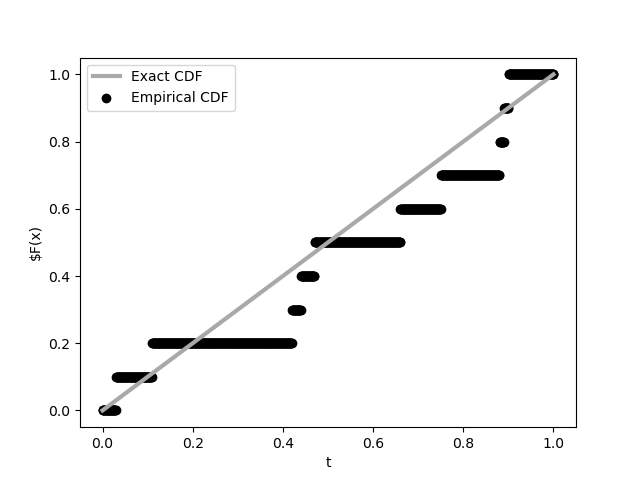
\includegraphics[width=2.5in]{STATS509/HW2/HW2Figures/problem3.png}
    \end{center}
    
    \item Code producing this output can be found at the end of this problem.
    \begin{lstlisting}[language=Python]
        KS statistic K=0.2194194194194194 at point t=0.4194194194194194
    \end{lstlisting}

\newpage
\lstinputlisting[language=Python]{HW2Code/problem2.py}
\end{enumerate}	
	
	
\newpage
\section*{Problem 4}
For each of the following, use the CDF approach to obtain the PDF of Y:
\begin{enumerate}
    \item $Y=2X$ if $X$ is a distributed exponential distribution. The exponential distribution is defined as:
    $$
    F(x;\lambda) = \begin{cases}
                    1-e^{-\lambda x} & x \ge 0, \\
                    0 & x < 0.
                    \end{cases}
    $$
    In a similar manner we can define $G(y)=P(Y\leq y)$ as the CDF of Y. Since CDF is just an integrated PDF we know we can recover the integrand, i.e. the PDF, by deriving $G$. First, since we are given the CDF of X, but not of Y we need to write out the explicit form of $G$:
    \begin{align*}
        G(y) &= P(Y\leq y) = P(2X \leq y) = P(X \leq y/2) = F(y/2) \\
        & = \begin{cases}
            1-e^{-\lambda y/2} & y \ge 0, \\
            0 & y < 0.
           \end{cases}
    \end{align*}
    Deriving case $y\ge 0$ we get:
    \begin{align*}
        g(y) &= \frac{\partial}{\partial y} G(y) = \frac{\partial}{\partial y} \left( 1-e^{-\frac{\lambda y}{2}} \right) \\
             &=  -e^{-\frac{\lambda y}{2}}  \frac{\partial}{\partial y} \left( -\lambda \frac{y}{2} \right) \\
             &= \frac{\lambda}{2} e^{-\frac{\lambda}{2}y}
    \end{align*}
    Finally we note that deriving the case $y,0$ retrieves just $0$. 
    
    \item $Y=-\ln{X}$ if $X$ is a Rectangular on $[0.1]$ I, again, assume Rectangular distribution is the Uniform distribution given by:
	$$ f(x)=\begin{cases}
            \frac{1}{b - a} & \mathrm{for}\ a \le x \le b, \\
            0 & \mathrm{for}\ x<a\ \mathrm{or}\ x>b
            \end{cases}
    $$
    whose CDF we determined in a previous problem as:
     $$ \F(t) = \int_{-\infty}^{\infty} f(t) dt = 
        \begin{cases}
            0 & \mathrm{for}\ t < 0 \\
            t & \mathrm{for}\ 0 \leq t \leq 1 \\
            1 & \mathrm{for}\  t > 1
        \end{cases}
    $$
    Again, write the CDF of $Y$ in terms of $F$ as:
    $$G(y) &= P(Y\leq y) = P(-\ln{X} \leq y) = P(\ln{X} \geq -y) = P(X \geq e^-y)$$
    Here we have to notice the complementarity $P(X\geq a) + P(X< a) = 1$ from which it follows that  $G(y) = 1 - P(X \leq e^{-y}) = 1 - F(e^{-y})$. Finally, we can write 
	$$ G(y)=\begin{cases}
            0& \mathrm{for}\ y \leq 0, \\
            1 - e^{-y} & \mathrm{for}\ y > 0
            \end{cases}
    $$
    Noting that differentiating first case will just produce $0$, we focus on the case $y>0$:
    \begin{align*}
        g(y) &= \frac{\partial}{\partial y} G(y) = \frac{\partial}{\partial y} \left( 1-e^{-y} \right) \\
             &=  e^{-y}
    \end{align*}
    
    \newpage
    \item $Y=X^2$ if X follows normal distribution. Again the trick is to find a clever way to write the CDF $G(y)$. The CDF of normal distribution can not be expressed using elementary functions and is instead given as an integral:
    $$F(x) = \frac 1 {\sqrt{2\pi}} \int_{-\infty}^x e^{-t^2/2} \, dt$$
    We can write $G$ as:
    \begin{align*}
        G(y) &= P(Y\leq y) = P(X^2 \leq y) = \\
             &= P(-\sqrt{y} \leq X \leq \sqrt{y}) \\
             &= P(X \leq \sqrt{y}) - P( X\leq -\sqrt{y}) = F(\sqrt{y}) - F(-\sqrt{y})
    \end{align*}
    Simply because it's just the way it is: 
    \begin{center}
        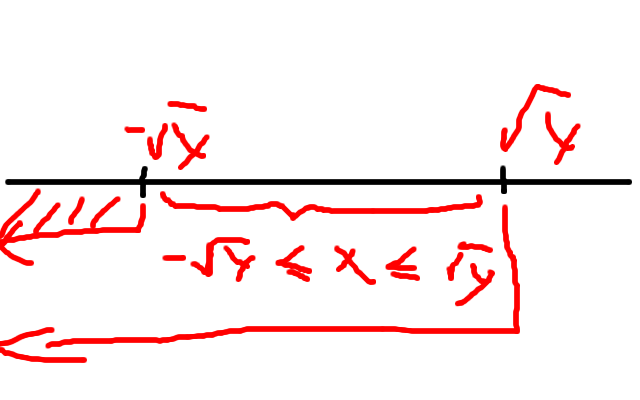
\includegraphics[width=1.5in]{HW2Figures/Picasso.png}
    \end{center}
    In addition to the ways things just are what they are it's also important to remember that the derivative of a CDF is just the PDF: $\partial_x F(x) = f(x)$, i.e. the normal distribution. Finally differentiating the CDF we have:
    \begin{align*}
        g(y) &= \frac{\partial}{\partial y} \left[F(\sqrt y) - F(- \sqrt y) \right] \\
             &=  \frac{\partial \sqrt y }{\partial y} \frac{\partial F(\sqrt y) }{\partial y} - \frac{\partial - \sqrt y}{\partial y} \frac{\partial F(- \sqrt y) }{\partial y} \\
             & = \frac{y^{-1/2}}{2} f(\sqrt y) -  \frac{y^{-1/2}}{2} f(-\sqrt y) \\
    \end{align*}
    Where we just applied the chain rule $\partial_x f(g(x)) = g'(x) f'(g(x))$. Since the normal distribution is symmetric around zero we can say that $f(\sqrt y) = f(-\sqrt y)$, pull the common factors out and simplify:
    $$g(y) = y^{-\frac{1}{2}} f(\sqrt y) = \frac{1}{\sqrt{2\pi y}}e^{-\frac{y}{2}} $$
\end{enumerate}

\newpage
\section*{Problem 5}
The code that produced the following plots is located at the end of the problem.
\begin{enumerate}
    \item 
    \begin{center}
    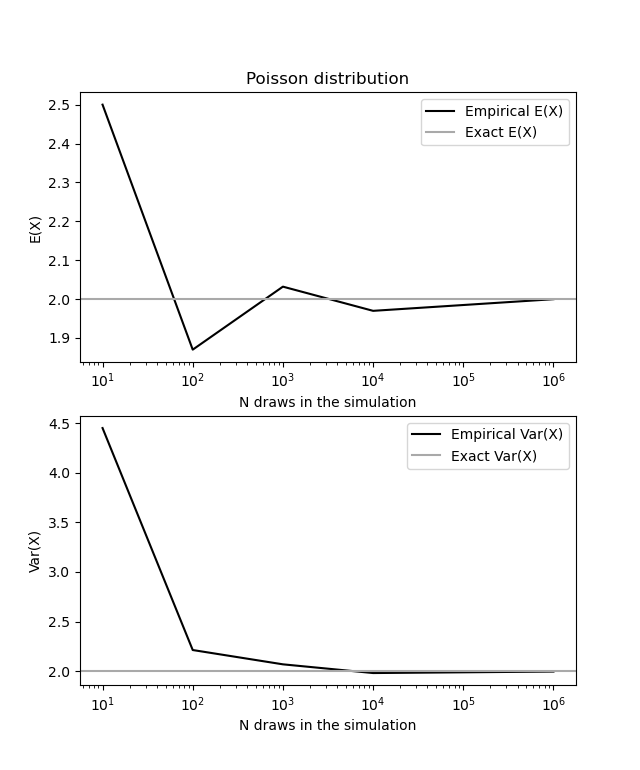
\includegraphics[width=3in]{STATS509/HW2/HW2Figures/problem5a.png}
    \end{center}
     \item 
    \begin{center}
    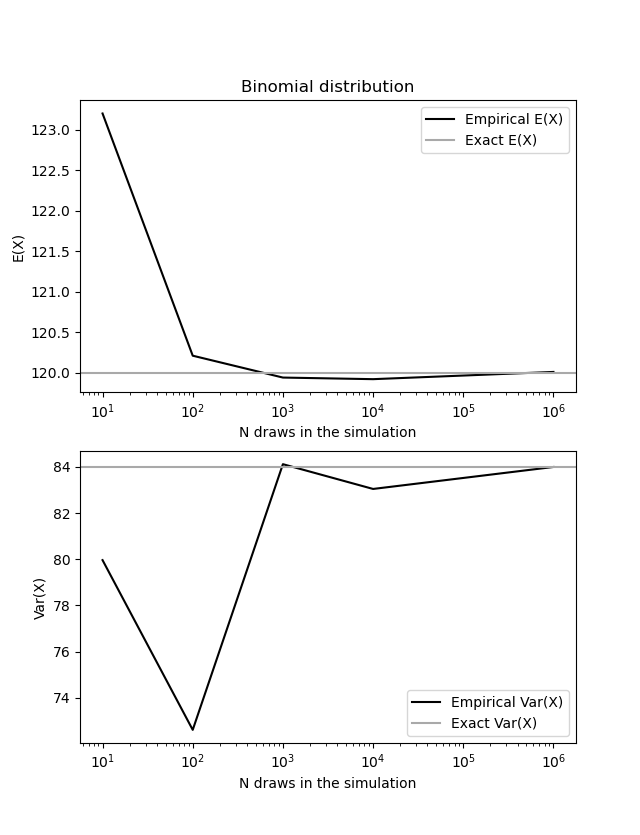
\includegraphics[width=3in]{STATS509/HW2/HW2Figures/problem5b.png}
    \end{center}
\end{enumerate}
\newpage
\lstinputlisting[language=Python]{HW2Code/problem5.py}



\newpage
\section*{Problem 6}
\begin{enumerate}
    \item From hint we know we have to focus on tossing the unfair coin twice. Then we have four possible outcomes $X=\{hh, ht, th, tt\}$. The probability of event $ht = p(1-p)$ could be different than 1/2 but the probabilities of $ht$ and $th$ will be equal. We can write then:
    $$P(ht \cup th) = P(ht) + P(th) - P(ht \cap th) = p(1-p) + (1-p)p = 2p(1-p)$$
    So while individual probabilities $P(ht)$ or $P(th)$ the probability to get an event from the smaller sample space $P(x|x \in X \cap hh \ cap tt) = P(X\in\{ht, th\})$ should be 1/2 (I might have mangled the notation a bit).
    
    \item 
    
    \item 
\end{enumerate}


\vspace{\baselineskip}
\noindent \textbf{\large 6.d}

The routine in the 6.c prints out the relevant numbers.  In 1000 trials my procedure produced 492 failures and 508 successes.  Seems pretty fair.  The mean number of attempts was 3.10 (two unfair coin tosses are required per attempt), which is near my calculated expectation at 3.125.

\vspace{\baselineskip}
\noindent \textbf{\large 7.a}

Discrete uniform, N = 9
\begin{align*}
E(X) &= \frac{N+1}{2} = 5 \\
V(X) &= \frac{N^2-1}{12} = 20/3
\end{align*}

\vspace{\baselineskip}
\noindent \textbf{\large 7.b}

Binomial, n=2, p=0.4

\begin{align*}
E(X) &= np = 0.8 \\
V(X) &= np(1-p) = 0.48
\end{align*}

\vspace{\baselineskip}
\noindent \textbf{\large 7.c}

Binomial, n=4, p=0.6

\begin{align*}
E(X) &= np = 2.4 \\
V(X) &= np(1-p) = 0.96
\end{align*}

\vspace{\baselineskip}
\noindent \textbf{\large 7.d}

Poisson $\lambda=3/2$

\begin{align*}
E(X) &= \lambda = 3/2 \\
V(X) &= \lambda = 3/2
\end{align*}

\vspace{\baselineskip}
\noindent \textbf{\large 7.e}

Rectangular on $[0,2]$

\begin{align*}
E(X) &= (a+b)/2 = 1 \\
V(X) &= (b-a)^2/12 = 1/3
\end{align*}

\vspace{\baselineskip}
\noindent \textbf{\large 7.f}

Exponential $\lambda=2$

\begin{align*}
E(X) &= 1/\lambda = 1/2 \\
V(X) &= 1/\lambda^2 = 1/4
\end{align*}

\vspace{\baselineskip}
\noindent \textbf{\large 7.g}

Power on $[0,1]$, $\theta=2$

\begin{align*}
E(X) &= \theta/(1+\theta) = 2/3 \\
V(X) &= \theta\left[ (1+\theta)^2(2+\theta)\right]^{-1} = 1/18
\end{align*}

\end{document}




\newpage
\section*{Problem 7}


\end{document}
